         \chapter{Sound}\fancyfoot[LO,RE]{Physics: Waves, Sound and Light}

    \setcounter{figure}{1}
    \setcounter{subfigure}{1}
    \label{9b5d72dd5f0585e544578ab90a9956a8}
         \section{Introduction}
    \nopagebreak
%            \label{m38799} $ \hspace{-5pt}\begin{array}{cccccccccccc}   \end{array} $ \hspace{2 pt}\raisebox{-0.2em}{
\includegraphics[height=1em]{../icons/www.pdf}} {(section shortcode: P10048 )} \par 
    \label{m38799*cid2}
\label{m38799*id183123}Have you ever thought about how amazing your sense of hearing is? It is actually pretty remarkable that we can hear the huge range of sounds and determine direction so quickly. How does something actually make a sound that you can hear? Anything that generates a disturbance in the air creates a pulse that travels away from the place where is was created. If this pulse enters your ear it can cause your ear drum to vibrate which is how you hear. If the source of the pulse creates a train of pulses then the disturbance is a wave.
\chapterstartvideo{VPdxu}
           
We generally say that sound is a wave. Sound waves are longitudinal, pressure waves, that means that the waves consists of compressions and rarefactions of the pressure of the air.\par 

\subsection*{Sound waves}
            \nopagebreak
A tuning fork is an instrument used by musicians to create sound waves of a specific frequency. They are often used to tune musical instruments.

\begin{minipage}{.5\textwidth}
      \label{m38783*id293458}Sound waves coming from a tuning fork are caused by the vibrations of the tuning fork which push against the air particles in front of it. As the air particles are pushed together a compression is formed. The particles behind the compression move further apart causing a rarefaction. As the particles continue to push against each other,
the sound wave travels through the air. Due to this motion of the particles, there is a constant variation in the pressure in the air. Sound waves are therefore pressure waves. This means that in media where the particles are closer together, sound waves will travel faster.
\mindsetvid{Science of sound}{VPdya}
\end{minipage}
\begin{minipage}{.5\textwidth}\begin{center}
\textbf{Tuning fork}\par
    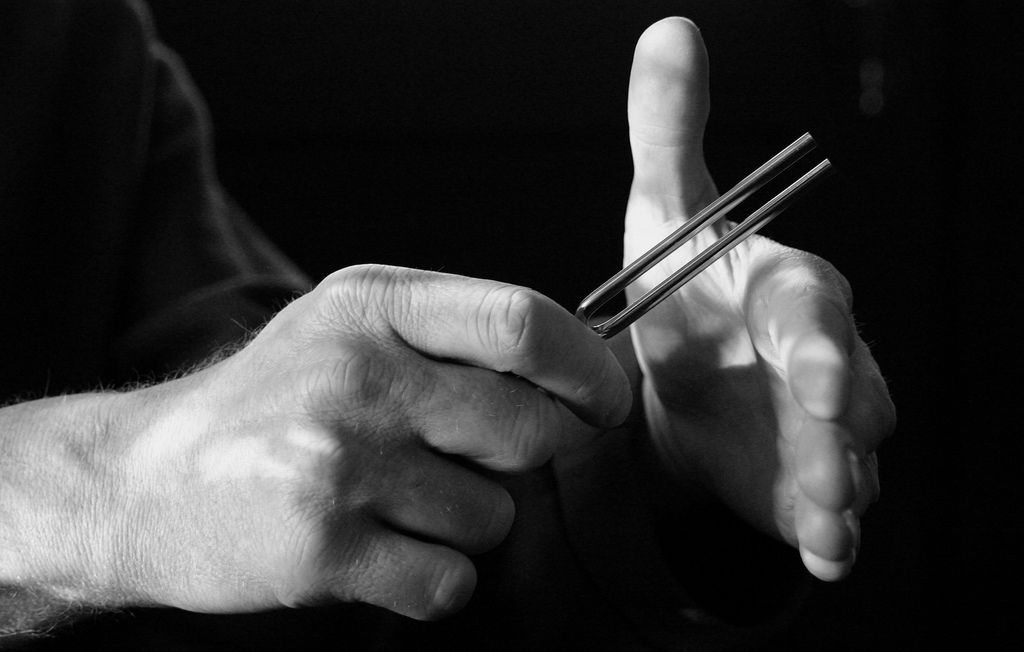
\includegraphics[width=0.8\textwidth]{photos/TuningFork2_Flickr_amonya.jpg}\par
\textit{Photo by amonya on Flickr.com}
\end{center}
\end{minipage}

      \label{m38783*id293466}Sound waves travel faster through liquids, like water, than through the air because water is denser than air (the particles are closer together). Sound waves travel faster in solids than in liquids.\par 
    \setcounter{subfigure}{0}
	\begin{figure}[H] % horizontal\label{m38783*uid18}
    \begin{center}
\scalebox{1} % Change this value to rescale the drawing.
{
\begin{pspicture}(0,-1.3159375)(10.862187,1.3159375)
\psline[linewidth=0.04cm](1.5942917,-0.29788056)(1.8169739,-0.30129474)
\psline[linewidth=0.04cm](1.8169739,-0.30129474)(1.8345535,0.44497925)
\psline[linewidth=0.04cm](1.9030713,0.44392854)(1.8835384,-0.3852649)
\psline[linewidth=0.04cm](1.8835384,-0.3852649)(1.7636325,-0.38342634)
\psline[linewidth=0.04cm](1.5771624,-0.29761782)(1.5947421,0.44865623)
\psline[linewidth=0.04cm](1.5262243,0.4497069)(1.5066916,-0.3794867)
\psline[linewidth=0.04cm](1.6437267,-0.38158786)(1.5238208,-0.37974924)
\psline[linewidth=0.04cm](1.6269228,-0.36750528)(1.6171566,-0.7821023)
\psline[linewidth=0.04cm](1.6171566,-0.7821023)(1.7541916,-0.7842031)
\psline[linewidth=0.04cm](1.7541916,-0.7842031)(1.7636325,-0.38342634)
\psline[linewidth=0.04cm](1.8345535,0.44497925)(1.9030713,0.44392854)
\psline[linewidth=0.04cm](1.5947421,0.44865623)(1.5262243,0.4497069)
\psdots[dotsize=0.04](2.0484376,0.2296875)
\psdots[dotsize=0.04](2.1284375,0.2496875)
\psdots[dotsize=0.04](2.0884376,0.2096875)
\psdots[dotsize=0.04](2.0084374,0.1296875)
\psdots[dotsize=0.04](2.1084375,0.0896875)
\psdots[dotsize=0.04](2.1684375,0.1696875)
\psdots[dotsize=0.04](2.1284375,0.1696875)
\psdots[dotsize=0.04](2.0684376,0.1296875)
\psdots[dotsize=0.04](2.0684376,-0.0103125)
\psdots[dotsize=0.04](2.1484375,-0.0303125)
\psdots[dotsize=0.04](2.1684375,0.1296875)
\psdots[dotsize=0.04](2.2684374,0.1896875)
\psdots[dotsize=0.04](2.2884376,0.1096875)
\psdots[dotsize=0.04](2.2884376,0.0096875)
\psdots[dotsize=0.04](2.2484374,-0.0103125)
\psdots[dotsize=0.04](2.1884375,-0.1103125)
\psdots[dotsize=0.04](2.0684376,-0.1503125)
\psdots[dotsize=0.04](1.9684376,-0.0903125)
\psdots[dotsize=0.04](2.0084374,-0.0103125)
\psdots[dotsize=0.04](2.1684375,-0.1103125)
\psdots[dotsize=0.04](2.2284374,-0.1503125)
\psdots[dotsize=0.04](2.2284374,0.0296875)
\psdots[dotsize=0.04](2.1884375,0.0896875)
\psdots[dotsize=0.04](2.2284374,0.2296875)
\psdots[dotsize=0.04](2.3084376,0.1696875)
\psdots[dotsize=0.04](2.3084376,-0.0703125)
\psdots[dotsize=0.04](2.2684374,-0.1303125)
\psdots[dotsize=0.04](2.1884375,-0.2103125)
\psdots[dotsize=0.04](2.1084375,-0.2103125)
\psdots[dotsize=0.04](2.0484376,-0.1703125)
\psdots[dotsize=0.04](1.9884375,-0.1903125)
\psdots[dotsize=0.04](2.0084374,-0.2103125)
\psdots[dotsize=0.04](2.0884376,-0.2303125)
\psdots[dotsize=0.04](2.1884375,-0.2903125)
\psdots[dotsize=0.04](2.2684374,-0.2303125)
\psdots[dotsize=0.04](2.3084376,-0.1303125)
\psdots[dotsize=0.04](2.3084376,0.0096875)
\psdots[dotsize=0.04](2.0484376,0.0496875)
\psdots[dotsize=0.04](2.0884376,-0.0903125)
\psdots[dotsize=0.04](2.0284376,-0.0703125)
\psdots[dotsize=0.04](2.2284374,0.1296875)
\psdots[dotsize=0.04](2.0084374,-0.2703125)
\psdots[dotsize=0.04](2.2684374,0.2496875)
\psdots[dotsize=0.04](2.3484375,0.2496875)
\psdots[dotsize=0.04](2.3484375,0.1696875)
\psdots[dotsize=0.04](2.4284375,0.2296875)
\psdots[dotsize=0.04](2.4084375,0.2296875)
\psdots[dotsize=0.04](2.4484375,0.0496875)
\psdots[dotsize=0.04](2.4284375,0.1496875)
\psdots[dotsize=0.04](2.3484375,0.1096875)
\psdots[dotsize=0.04](2.3684375,0.0096875)
\psdots[dotsize=0.04](2.3684375,0.0096875)
\psdots[dotsize=0.04](2.3084376,0.0496875)
\psdots[dotsize=0.04](2.4484375,-0.0903125)
\psdots[dotsize=0.04](2.3684375,-0.1303125)
\psdots[dotsize=0.04](2.3284376,-0.1103125)
\psdots[dotsize=0.04](2.4084375,-0.0703125)
\psdots[dotsize=0.04](2.4684374,-0.0303125)
\psdots[dotsize=0.04](2.4684374,-0.1503125)
\psdots[dotsize=0.04](2.4284375,-0.1903125)
\psdots[dotsize=0.04](2.3484375,-0.2303125)
\psdots[dotsize=0.04](2.3084376,-0.2503125)
\psdots[dotsize=0.04](2.3884375,-0.2903125)
\psdots[dotsize=0.04](2.4884374,-0.2503125)
\psdots[dotsize=0.04](2.2284374,-0.0503125)
\psdots[dotsize=0.04](2.1084375,-0.2903125)
\psdots[dotsize=0.04](2.0084374,0.0696875)
\psdots[dotsize=0.04](2.0084374,0.2296875)
\psdots[dotsize=0.04](2.0484376,0.2696875)
\psdots[dotsize=0.04](2.4484375,0.1496875)
\psdots[dotsize=0.04](2.4684374,0.2296875)
\psdots[dotsize=0.04](2.5484376,0.2296875)
\psdots[dotsize=0.04](2.7284374,0.1896875)
\psdots[dotsize=0.04](2.7684374,-0.0703125)
\psdots[dotsize=0.04](2.5884376,-0.0103125)
\psdots[dotsize=0.04](2.6684375,0.1096875)
\psdots[dotsize=0.04](2.8684375,0.0296875)
\psdots[dotsize=0.04](3.3084376,-0.0903125)
\psdots[dotsize=0.04](3.1484375,0.0896875)
\psdots[dotsize=0.04](2.9884374,0.1296875)
\psdots[dotsize=0.04](3.0084374,0.1896875)
\psdots[dotsize=0.04](3.2084374,0.1696875)
\psdots[dotsize=0.04](2.8084376,0.2696875)
\psdots[dotsize=0.04](3.0684376,-0.0703125)
\psdots[dotsize=0.04](2.6284375,-0.2303125)
\psdots[dotsize=0.04](2.7884376,-0.2703125)
\psdots[dotsize=0.04](3.0284376,-0.2503125)
\psdots[dotsize=0.04](2.9084375,-0.0903125)
\psdots[dotsize=0.04](3.2284374,-0.2503125)
\psdots[dotsize=0.04](3.2684374,0.0296875)
\psdots[dotsize=0.04](3.1284375,0.2496875)
\psdots[dotsize=0.04](3.3284376,0.2496875)
\psdots[dotsize=0.04](3.4884374,0.2096875)
\psdots[dotsize=0.04](3.6884375,0.2496875)
\psdots[dotsize=0.04](3.6484375,0.0696875)
\psdots[dotsize=0.04](3.6084375,-0.1103125)
\psdots[dotsize=0.04](3.3484375,0.0496875)
\psdots[dotsize=0.04](3.4884374,0.0696875)
\psdots[dotsize=0.04](3.4484375,-0.1703125)
\psdots[dotsize=0.04](3.3284376,-0.2303125)
\psdots[dotsize=0.04](3.5484376,-0.2703125)
\psdots[dotsize=0.04](3.6684375,-0.2703125)
\psdots[dotsize=0.04](3.7884376,0.2496875)
\psdots[dotsize=0.04](3.8684375,0.2696875)
\psdots[dotsize=0.04](3.8284376,0.2296875)
\psdots[dotsize=0.04](3.7484374,0.1496875)
\psdots[dotsize=0.04](3.8484375,0.1096875)
\psdots[dotsize=0.04](3.9084375,0.1896875)
\psdots[dotsize=0.04](3.8684375,0.1896875)
\psdots[dotsize=0.04](3.8084376,0.1496875)
\psdots[dotsize=0.04](3.8084376,0.0096875)
\psdots[dotsize=0.04](3.8884375,-0.0103125)
\psdots[dotsize=0.04](3.9084375,0.1496875)
\psdots[dotsize=0.04](4.0084376,0.2096875)
\psdots[dotsize=0.04](4.0284376,0.1296875)
\psdots[dotsize=0.04](4.0284376,0.0296875)
\psdots[dotsize=0.04](3.9884374,0.0096875)
\psdots[dotsize=0.04](3.9284375,-0.0903125)
\psdots[dotsize=0.04](3.8084376,-0.1303125)
\psdots[dotsize=0.04](3.7084374,-0.0703125)
\psdots[dotsize=0.04](3.7484374,0.0096875)
\psdots[dotsize=0.04](3.9084375,-0.0903125)
\psdots[dotsize=0.04](3.9684374,-0.1303125)
\psdots[dotsize=0.04](3.9684374,0.0496875)
\psdots[dotsize=0.04](3.9284375,0.1096875)
\psdots[dotsize=0.04](3.9684374,0.2496875)
\psdots[dotsize=0.04](4.0484376,0.1896875)
\psdots[dotsize=0.04](4.0484376,-0.0503125)
\psdots[dotsize=0.04](4.0084376,-0.1103125)
\psdots[dotsize=0.04](3.9284375,-0.1903125)
\psdots[dotsize=0.04](3.8484375,-0.1903125)
\psdots[dotsize=0.04](3.7884376,-0.1503125)
\psdots[dotsize=0.04](3.7284374,-0.1703125)
\psdots[dotsize=0.04](3.7484374,-0.1903125)
\psdots[dotsize=0.04](3.8284376,-0.2103125)
\psdots[dotsize=0.04](3.9284375,-0.2703125)
\psdots[dotsize=0.04](4.0084376,-0.2103125)
\psdots[dotsize=0.04](4.0484376,-0.1103125)
\psdots[dotsize=0.04](4.0484376,0.0296875)
\psdots[dotsize=0.04](3.7884376,0.0696875)
\psdots[dotsize=0.04](3.8284376,-0.0703125)
\psdots[dotsize=0.04](3.7684374,-0.0503125)
\psdots[dotsize=0.04](3.9684374,0.1496875)
\psdots[dotsize=0.04](3.7484374,-0.2503125)
\psdots[dotsize=0.04](4.0084376,0.2696875)
\psdots[dotsize=0.04](4.0884376,0.2696875)
\psdots[dotsize=0.04](4.0884376,0.1896875)
\psdots[dotsize=0.04](4.1684375,0.2496875)
\psdots[dotsize=0.04](4.1484375,0.2496875)
\psdots[dotsize=0.04](4.1884375,0.0696875)
\psdots[dotsize=0.04](4.1684375,0.1696875)
\psdots[dotsize=0.04](4.0884376,0.1296875)
\psdots[dotsize=0.04](4.1084375,0.0296875)
\psdots[dotsize=0.04](4.1084375,0.0296875)
\psdots[dotsize=0.04](4.0484376,0.0696875)
\psdots[dotsize=0.04](4.1884375,-0.0703125)
\psdots[dotsize=0.04](4.1084375,-0.1103125)
\psdots[dotsize=0.04](4.0684376,-0.0903125)
\psdots[dotsize=0.04](4.1484375,-0.0503125)
\psdots[dotsize=0.04](4.2084374,-0.0103125)
\psdots[dotsize=0.04](4.2084374,-0.1303125)
\psdots[dotsize=0.04](4.1684375,-0.1703125)
\psdots[dotsize=0.04](4.0884376,-0.2103125)
\psdots[dotsize=0.04](4.0484376,-0.2303125)
\psdots[dotsize=0.04](4.1284375,-0.2703125)
\psdots[dotsize=0.04](4.2284374,-0.2303125)
\psdots[dotsize=0.04](3.9684374,-0.0303125)
\psdots[dotsize=0.04](3.8484375,-0.2703125)
\psdots[dotsize=0.04](3.7484374,0.0896875)
\psdots[dotsize=0.04](3.7484374,0.2496875)
\psdots[dotsize=0.04](3.7884376,0.2896875)
\psdots[dotsize=0.04](4.1884375,0.1696875)
\psdots[dotsize=0.04](4.2084374,0.2496875)
\psdots[dotsize=0.04](4.2884374,0.2496875)
\psdots[dotsize=0.04](4.4684377,0.2096875)
\psdots[dotsize=0.04](4.5084376,-0.0503125)
\psdots[dotsize=0.04](4.3284373,0.0096875)
\psdots[dotsize=0.04](4.4084377,0.1296875)
\psdots[dotsize=0.04](4.6084375,0.0496875)
\psdots[dotsize=0.04](5.0484376,-0.0703125)
\psdots[dotsize=0.04](4.8884373,0.1096875)
\psdots[dotsize=0.04](4.7284374,0.1496875)
\psdots[dotsize=0.04](4.7484374,0.2096875)
\psdots[dotsize=0.04](4.9484377,0.1896875)
\psdots[dotsize=0.04](4.5484376,0.2896875)
\psdots[dotsize=0.04](4.8084373,-0.0503125)
\psdots[dotsize=0.04](4.3684373,-0.2103125)
\psdots[dotsize=0.04](4.5284376,-0.2503125)
\psdots[dotsize=0.04](4.7684374,-0.2303125)
\psdots[dotsize=0.04](4.6484375,-0.0703125)
\psdots[dotsize=0.04](4.9684377,-0.2303125)
\psdots[dotsize=0.04](5.0084376,0.0496875)
\psdots[dotsize=0.04](4.8684373,0.2696875)
\psdots[dotsize=0.04](5.0684376,0.2696875)
\psdots[dotsize=0.04](5.2284374,0.2296875)
\psdots[dotsize=0.04](5.4284377,0.2696875)
\psdots[dotsize=0.04](5.3884373,0.0896875)
\psdots[dotsize=0.04](5.3484373,-0.0903125)
\psdots[dotsize=0.04](5.0884376,0.0696875)
\psdots[dotsize=0.04](5.2284374,0.0896875)
\psdots[dotsize=0.04](5.1884375,-0.1503125)
\psdots[dotsize=0.04](5.0684376,-0.2103125)
\psdots[dotsize=0.04](5.2884374,-0.2503125)
\psdots[dotsize=0.04](5.4084377,-0.2503125)
\psdots[dotsize=0.04](5.5084376,0.2296875)
\psdots[dotsize=0.04](5.5884376,0.2496875)
\psdots[dotsize=0.04](5.5484376,0.2096875)
\psdots[dotsize=0.04](5.4684377,0.1296875)
\psdots[dotsize=0.04](5.5684376,0.0896875)
\psdots[dotsize=0.04](5.6284375,0.1696875)
\psdots[dotsize=0.04](5.5884376,0.1696875)
\psdots[dotsize=0.04](5.5284376,0.1296875)
\psdots[dotsize=0.04](5.5284376,-0.0103125)
\psdots[dotsize=0.04](5.6084375,-0.0303125)
\psdots[dotsize=0.04](5.6284375,0.1296875)
\psdots[dotsize=0.04](5.7284374,0.1896875)
\psdots[dotsize=0.04](5.7484374,0.1096875)
\psdots[dotsize=0.04](5.7484374,0.0096875)
\psdots[dotsize=0.04](5.7084374,-0.0103125)
\psdots[dotsize=0.04](5.6484375,-0.1103125)
\psdots[dotsize=0.04](5.5284376,-0.1503125)
\psdots[dotsize=0.04](5.4284377,-0.0903125)
\psdots[dotsize=0.04](5.4684377,-0.0103125)
\psdots[dotsize=0.04](5.6284375,-0.1103125)
\psdots[dotsize=0.04](5.6884375,-0.1503125)
\psdots[dotsize=0.04](5.6884375,0.0296875)
\psdots[dotsize=0.04](5.6484375,0.0896875)
\psdots[dotsize=0.04](5.6884375,0.2296875)
\psdots[dotsize=0.04](5.7684374,0.1696875)
\psdots[dotsize=0.04](5.7684374,-0.0703125)
\psdots[dotsize=0.04](5.7284374,-0.1303125)
\psdots[dotsize=0.04](5.6484375,-0.2103125)
\psdots[dotsize=0.04](5.5684376,-0.2103125)
\psdots[dotsize=0.04](5.5084376,-0.1703125)
\psdots[dotsize=0.04](5.4484377,-0.1903125)
\psdots[dotsize=0.04](5.4684377,-0.2103125)
\psdots[dotsize=0.04](5.5484376,-0.2303125)
\psdots[dotsize=0.04](5.6484375,-0.2903125)
\psdots[dotsize=0.04](5.7284374,-0.2303125)
\psdots[dotsize=0.04](5.7684374,-0.1303125)
\psdots[dotsize=0.04](5.7684374,0.0096875)
\psdots[dotsize=0.04](5.5084376,0.0496875)
\psdots[dotsize=0.04](5.5484376,-0.0903125)
\psdots[dotsize=0.04](5.4884377,-0.0703125)
\psdots[dotsize=0.04](5.6884375,0.1296875)
\psdots[dotsize=0.04](5.4684377,-0.2703125)
\psdots[dotsize=0.04](5.7284374,0.2496875)
\psdots[dotsize=0.04](5.8084373,0.2496875)
\psdots[dotsize=0.04](5.8084373,0.1696875)
\psdots[dotsize=0.04](5.8884373,0.2296875)
\psdots[dotsize=0.04](5.8684373,0.2296875)
\psdots[dotsize=0.04](5.9084377,0.0496875)
\psdots[dotsize=0.04](5.8884373,0.1496875)
\psdots[dotsize=0.04](5.8084373,0.1096875)
\psdots[dotsize=0.04](5.8284373,0.0096875)
\psdots[dotsize=0.04](5.8284373,0.0096875)
\psdots[dotsize=0.04](5.7684374,0.0496875)
\psdots[dotsize=0.04](5.9084377,-0.0903125)
\psdots[dotsize=0.04](5.8284373,-0.1303125)
\psdots[dotsize=0.04](5.7884374,-0.1103125)
\psdots[dotsize=0.04](5.8684373,-0.0703125)
\psdots[dotsize=0.04](5.9284377,-0.0303125)
\psdots[dotsize=0.04](5.9284377,-0.1503125)
\psdots[dotsize=0.04](5.8884373,-0.1903125)
\psdots[dotsize=0.04](5.8084373,-0.2303125)
\psdots[dotsize=0.04](5.7684374,-0.2503125)
\psdots[dotsize=0.04](5.8484373,-0.2903125)
\psdots[dotsize=0.04](5.9484377,-0.2503125)
\psdots[dotsize=0.04](5.6884375,-0.0503125)
\psdots[dotsize=0.04](5.5684376,-0.2903125)
\psdots[dotsize=0.04](5.4684377,0.0696875)
\psdots[dotsize=0.04](5.4684377,0.2296875)
\psdots[dotsize=0.04](5.5084376,0.2696875)
\psdots[dotsize=0.04](5.9084377,0.1496875)
\psdots[dotsize=0.04](5.9284377,0.2296875)
\psdots[dotsize=0.04](6.0084376,0.2296875)
\psdots[dotsize=0.04](6.1884375,0.1896875)
\psdots[dotsize=0.04](6.2284374,-0.0703125)
\psdots[dotsize=0.04](6.0484376,-0.0103125)
\psdots[dotsize=0.04](6.1284375,0.1096875)
\psdots[dotsize=0.04](6.3284373,0.0296875)
\psdots[dotsize=0.04](6.7684374,-0.0903125)
\psdots[dotsize=0.04](6.6084375,0.0896875)
\psdots[dotsize=0.04](6.4484377,0.1296875)
\psdots[dotsize=0.04](6.4684377,0.1896875)
\psdots[dotsize=0.04](6.6684375,0.1696875)
\psdots[dotsize=0.04](6.2684374,0.2696875)
\psdots[dotsize=0.04](6.5284376,-0.0703125)
\psdots[dotsize=0.04](6.0884376,-0.2303125)
\psdots[dotsize=0.04](6.2484374,-0.2703125)
\psdots[dotsize=0.04](6.4884377,-0.2503125)
\psdots[dotsize=0.04](6.3684373,-0.0903125)
\psdots[dotsize=0.04](6.6884375,-0.2503125)
\psdots[dotsize=0.04](6.7284374,0.0296875)
\psdots[dotsize=0.04](6.5884376,0.2496875)
\psdots[dotsize=0.04](6.7884374,0.2496875)
\psdots[dotsize=0.04](6.9484377,0.2096875)
\psdots[dotsize=0.04](7.1484375,0.2496875)
\psdots[dotsize=0.04](7.1084375,0.0696875)
\psdots[dotsize=0.04](7.0684376,-0.1103125)
\psdots[dotsize=0.04](6.8084373,0.0496875)
\psdots[dotsize=0.04](6.9484377,0.0696875)
\psdots[dotsize=0.04](6.9084377,-0.1703125)
\psdots[dotsize=0.04](6.7884374,-0.2303125)
\psdots[dotsize=0.04](7.0084376,-0.2703125)
\psdots[dotsize=0.04](7.1284375,-0.2703125)
\rput(4.0528126,-1.1053125){\small compressions}
\psline[linewidth=0.04cm](3.9484375,-0.9903125)(3.9484375,-0.6303125)
\psline[linewidth=0.04cm](2.2484374,-0.6303125)(5.7484374,-0.6303125)
\psline[linewidth=0.04cm,arrowsize=0.05291667cm 2.0,arrowlength=1.4,arrowinset=0.4]{->}(2.2684374,-0.6303125)(2.2884376,-0.3303125)
\psline[linewidth=0.04cm,arrowsize=0.05291667cm 2.0,arrowlength=1.4,arrowinset=0.4]{->}(3.9484375,-0.6103125)(3.9684374,-0.3103125)
\psline[linewidth=0.04cm,arrowsize=0.05291667cm 2.0,arrowlength=1.4,arrowinset=0.4]{->}(5.7284374,-0.6303125)(5.7484374,-0.3303125)
\psline[linewidth=0.04cm](4.7284374,0.9896875)(4.7284374,0.6296875)
\psline[linewidth=0.04cm](3.0284376,0.6296875)(6.5284376,0.6296875)
\psline[linewidth=0.04cm,arrowsize=0.05291667cm 2.0,arrowlength=1.4,arrowinset=0.4]{->}(3.0484376,0.6296875)(3.0684376,0.3296875)
\psline[linewidth=0.04cm,arrowsize=0.05291667cm 2.0,arrowlength=1.4,arrowinset=0.4]{->}(4.7284374,0.6096875)(4.7484374,0.3096875)
\psline[linewidth=0.04cm,arrowsize=0.05291667cm 2.0,arrowlength=1.4,arrowinset=0.4]{->}(6.5084376,0.6296875)(6.5284376,0.3296875)
\rput(4.685625,1.1146874){\small rarefactions}
\rput(0.48132812,0.546875){\small vibrating}
\rput(0.5132812,0.2346875){\small tuning}
\rput(0.4678125,-0.1053125){\small fork}
\psline[linewidth=0.04cm](0.9284375,0.0096875)(1.4084375,0.0096875)
\rput(9.066093,0.2146875){\small column of air in front}
\rput(9.035313,-0.1053125){\small of tuning fork}
\end{pspicture}
}
\end{center}
\caption{Sound waves are pressure waves and need a medium through which to travel.}
 \end{figure}       

\Tip{A sound wave is a pressure wave. This means that regions of high pressure (compressions) and low pressure (rarefactions) are created as the sound source vibrates. These compressions and rarefactions arise because the source vibrates longitudinally and the longitudinal motion of air produces pressure fluctuations.}
	
\begin{activity}{Build your own telephone} 
Have you ever wondered if you can actually use tin cans or cups to make a telephone? Try it and see!

What you need:
\begin{itemize}
 \item Two tin cans or paper paper cups
  \item String
  \item Toothpicks or small sticks
\end{itemize}

Try This:
\begin{enumerate}[noitemsep, label=\textbf{\arabic*}. ] 
\item Tie a toothpick on each end of a length of string.
\item Make a hole in the base of the can or cup. Poke the toothpick through the end of the can. Pull the string tight so the toothpick rests on the inside bottom of the can. Put one can at each end of the string. (You may want to experiment with different cans or cups and strings or wires to see what works best.)
\item Hold the string tight and talk into one of the cans. The person at the other end should be able to hear you. Why does the string have to be tight?
\item Try to make a party line by tying a third string and can or cup onto the middle of the string. Can everybody talk to everybody else?
\end{enumerate}

Sound waves need something to travel through. Usually they travel through air, but they can travel much faster and farther through a string. The string has to be tight or else the sound wave cannot travel through it. The cup helps to amplify the sound on the other end. 
\end{activity}

    \label{m38799*cid3}
            \section{Speed of sound}
            \nopagebreak
      \label{m38799*id183885}The speed of sound depends on the medium the sound is travelling in. Sound travels faster in solids than in liquids, and faster in liquids than in gases. This is because the density of solids is higher than that of liquids which means that the particles are closer together. Sound can be transmitted more easily.\par 
\mindsetvid{Speed of sound}{VPeac}
\begin{minipage}[t]{.5\textwidth}
      \label{m38799*id183891}The speed of sound also depends on the temperature of the medium. The hotter the medium is, the faster its particles move and therefore the quicker the sound will travel through the medium. When we heat a substance, the particles in that substance have more kinetic energy and vibrate or move faster. Sound can therefore be transmitted more easily and quickly in hotter substances.\\

 
      \label{m38799*id183897}Sound waves are pressure waves. The speed of sound will therefore be influenced by the pressure of the medium through which it is travelling. At sea level the air pressure is higher than high up on a mountain. Sound will travel faster at sea level where the air pressure is higher than it would at places high above sea level.\par 
\end{minipage}
\begin{minipage}[t]{.5\textwidth}
\begin{center}
\begin{table}[H]
\centering
 \begin{tabular}{|c|c|}\hline
Substance	& $v$ ($\text{m}\cdot \text{s}^{-1}$)\\ \hline \hline
aluminium	&6420 \\ \hline
brick	&3650 \\ \hline
copper	&4760	 	 \\ \hline
glass &5100	 \\ \hline 	 	 
gold	&3240	 \\ \hline 	
lead	&2160	 \\ \hline 
water, sea	&1531 \\ \hline
air, 0 $^o$C&331 \\ \hline
air, 20 $^o$C&343 \\ \hline
\end{tabular}
\caption{The speed of sound in different materials.}
\end{table}
\end{center}
\end{minipage}


\IFact{The speed of sound in air, at sea level, at a temperature of $21{}^{\circ }\text{C}$ and under normal atmospheric conditions, is $344\phantom{\rule{2pt}{0ex}}\text{m}\ensuremath{\cdot}\text{s}{}^{-1}$.} 

\begin{i_experiment}{Measuring the speed of sound in air}
\textbf{Aim:} To measure the speed of sound.

\textbf{Apparatus:} 
\begin{itemize}
 \item Starter's gun or anything that can produce a loud sound in response to visible action
  \item Stopwatch
  \end{itemize}

\textbf{Method:} The speed of sound can be measured because light travels much faster than sound. Light travels at about 300 000 $\text{m}\cdot\text{s}^{-1}$ (you will learn more about the speed of light in the next chapter) while sound only travels at about 300 $\text{m}\cdot\text{s}^{-1}$.  This difference means that over a distance of 300 $\text{m}$, the light from an event will reach your eyes almost instantly but there will be an approximate half a second lag before you hear the sound produced.  Thus if a starter's pistol is fired from a great distance, you will see the smoke immediately but there will be a lag before you hear the sound.  If you know the distance and the time then you can calculate the speed (distance divided by time). You don't need a gun but anything that you can see producing a loud sound.

Try this:
\begin{enumerate}[noitemsep, label=\textbf{\arabic*}. ] 
\item Find a place where you know the precise, straight-line distance between two points (maybe an athletics track)
\item Someone needs to stand at the one point to produce the sound 
\item Another person needs to stand at the other point with the stop watches
\item The person with the stopwatch should start the stopwatch when they see the other person make the sound and stop the stopwatch when they hear the sound (do this a few times and write the times down)
\end{enumerate}
\textbf{Results:}

\begin{minipage}{.45\textwidth}
You can now calculate the speed to sound by dividing the distance by the time. Remember to work in S.I. units (metres and seconds). If you took multiple readings then you can sum them and divide by the number of readings to get an average time reading. Use the average time to calculate the speed:
\begin{equation*}
 v = \frac{D}{t}
\end{equation*} 
\end{minipage}\hspace{.03\textwidth}
\begin{minipage}{.5\textwidth}
\begin{table}[H]
 \begin{tabular}{|c|c|c|}\hline\hline
Time (s) & Distance (m) & $v~(\text{m}\cdot\text{s}^{-1})$ \\\hline
 & & \\\hline 
 & & \\\hline 
 & & \\\hline 
 & & \\\hline 
 & & \\\hline 
 & & \\\hline \hline
\multicolumn{3}{|c|}{Averages} \\ \hline
 & & \\\hline 
 \end{tabular}
\end{table}
\end{minipage}\\
\textbf{Conclusions:}
Some questions to ask:
\begin{itemize}
 \item What is your reaction time on the stopwatch? You can test this by starting it and then trying to stop it immediately.
 \item What was the forecast temperature on the day of the measurement?
 \item Was it humid or very dry?
\end{itemize}

Discuss what might change the speed of sound that you measured.

You can vary this experiment by trying it on days when the weather is different as this can change air pressure and temperature. \end{i_experiment}

\subsection{Reflection and echoes}

When the sound waves collide with an object they are reflected. You can think of the individual particles that are oscillating about their equilibrium position colliding into the object when the wave passes. They bounce off the object causing the wave to be reflected.

In a space with many small objects there are reflections at every surface but they are too small and too mixed up to have an outcome that a human can hear. However, when there is an open space that has only large surfaces, for example a school hall that is empty, then the reflected sound can actually be heard. The sound wave is reflected in such a wave that the wave looks the same but is moving in the opposite direction.
\mindsetvid{Reflection and echoes}{VPebb}

This means that if you stand in a hall and loudly say ``hello'' you will hear yourself say ``hello'' a split second later. This is an echo. This can also happen outdoors in a wide open space with a large reflecting surface nearby, like standing near a mountain cliff in an area with no trees or bushes.

This is a very useful property of waves.

         \subsection*{SONAR}
            \nopagebreak
      \label{m38800*id185202}
\begin{minipage}{.5\textwidth}
      	\begin{figure}[H] % horizontal\label{m38800*id185205}
    \begin{center}

\includegraphics[width=.8\textwidth]{photos/sonar_NOAANationalOceanService_flickr.jpg}
% 
% \scalebox{0.8} % Change this value to rescale the drawing.
% {
% \begin{pspicture}(0,-3.93)(11.42,3.91)
% \definecolor{color78b}{rgb}{0.6,0.6,0.6}
% \psbezier[linewidth=0.04](0.52,-1.6283582)(3.3282945,-0.05)(4.980751,-1.0964925)(5.8,-2.11)(6.619249,-3.1235075)(8.99,-3.91)(10.64,-3.71)
% \psbezier[linewidth=0.04,fillstyle=solid,fillcolor=color78b](1.94,2.61)(1.9801459,1.77)(1.84,1.17)(2.44,1.15)(3.04,1.13)(6.68,1.01)(7.358321,1.29)(8.036642,1.57)(9.52,2.81)(8.58,2.59)(7.64,2.37)(1.96,2.43)(1.92,2.59)
% \psline[linewidth=0.04cm](2.52,2.49)(2.52,3.27)
% \psline[linewidth=0.04cm](2.52,3.27)(4.44,3.27)
% \psline[linewidth=0.04cm](4.44,3.27)(4.44,2.45)
% \psline[linewidth=0.04cm](3.14,3.81)(3.14,3.27)
% \psline[linewidth=0.04cm](3.76,3.81)(3.76,3.27)
% \psellipse[linewidth=0.04,dimen=outer](3.45,3.82)(0.33,0.09)
% \pscircle[linewidth=0.04,dimen=outer,fillstyle=solid,fillcolor=color78b](2.74,3.05){0.14}
% \pscircle[linewidth=0.04,dimen=outer,fillstyle=solid,fillcolor=color78b](3.18,3.05){0.14}
% \pscircle[linewidth=0.04,dimen=outer,fillstyle=solid,fillcolor=color78b](3.7,3.05){0.14}
% \pscircle[linewidth=0.04,dimen=outer,fillstyle=solid,fillcolor=color78b](4.12,3.05){0.14}
% \pscircle[linewidth=0.04,dimen=outer,fillstyle=solid,fillcolor=color78b](2.96,2.77){0.14}
% \pscircle[linewidth=0.04,dimen=outer,fillstyle=solid,fillcolor=color78b](3.44,2.77){0.14}
% \pscircle[linewidth=0.04,dimen=outer,fillstyle=solid,fillcolor=color78b](3.9,2.75){0.14}
% \rput(7.5798435,2.24){SAS Sonar}
% \psframe[linewidth=0.04,dimen=outer,fillstyle=solid](3.24,1.15)(3.02,1.05)
% \psframe[linewidth=0.04,dimen=outer,fillstyle=solid](4.58,1.13)(4.36,1.03)
% \pscustom[linewidth=0.04]
% {
% \newpath
% \moveto(9.94,1.31)
% }
% \psline[linewidth=0.04cm](0.0,1.61)(11.4,1.61)
% \psline[linewidth=0.04cm](3.12,1.15)(3.76,-0.85)
% \psline[linewidth=0.04cm](3.76,-0.85)(4.48,1.13)
% \psline[linewidth=0.04cm](3.2972062,0.25496995)(3.4476187,0.11434252)
% \psline[linewidth=0.04cm](3.4476187,0.11434252)(3.4875562,0.316345)
% \psline[linewidth=0.04cm](4.229458,0.10226333)(4.187863,0.30393106)
% \psline[linewidth=0.04cm](4.187863,0.30393106)(4.0386105,0.1620733)
% \rput(3.2217188,-1.2){seabed}
% \rput(1.949375,0.62){transmitter}
% \rput(5.47,0.62){receiver}
% \psline[linewidth=0.04cm,arrowsize=0.05291667cm 2.0,arrowlength=1.4,arrowinset=0.4]{->}(2.56,0.81)(3.0,1.03)
% \psline[linewidth=0.04cm,arrowsize=0.05291667cm 2.0,arrowlength=1.4,arrowinset=0.4]{->}(4.92,0.79)(4.64,1.03)
% %\psline[linewidth=0.04cm,arrowsize=0.05291667cm %2.0,arrowlength=1.4,arrowinset=0.4]{->}(6.36,-0.09)(6.36,-0.09)
% \rput(7.020781,-0.46){sea}
% \end{pspicture}
% }
\end{center}

 \end{figure}       
\end{minipage}
\begin{minipage}{.5\textwidth}
      \label{m38800*id185212}Ships on the ocean make use of the reflecting properties of sound waves to determine the depth of the ocean. A sound wave is transmitted and bounces off the seabed. Because the speed of sound is known and the time lapse between sending and receiving the sound can be measured, the distance from the ship to the bottom of the ocean can be determined, This is called sonar, which is an acronym for \textbf{So}und \textbf{N}avigation \textbf{A}nd \textbf{R}anging.\par 
      \label{m38800*uid13}
     \end{minipage}
            

\begin{wex}{SONAR}{A ship sends a signal to the bottom of the ocean to determine the depth of the ocean. The speed of sound in sea water is 1450 $\text{m}\cdot\text{s}^{-1}$ If the signal is received 1,5 seconds later, how deep is the ocean at that point?}{
\westep{Identify what is given and what is being asked:}
\begin{eqnarray*}
s &=& 1450 \ \text{m}.\text{s}^{-1}\\
t &=& 1,5 \ \text{s} \ \text{there \ and \ back}\\
\therefore t &= & 0,75 \ \text{s} \ \text{one \ way}\\
d &=& ?
\end{eqnarray*}

\westep{Calculate the distance:}
\begin{eqnarray*}
\text{Distance} &=& \text{speed} \times \text{time} \\
D &=& s \times t \\
&=& 1450~\text{m}\cdot\text{s}^{-1} \times 0,75 s \\
&=& 1087,5 \ \text{m}
\end{eqnarray*}
}\end{wex}
 
\subsection{Echolocation}
            \nopagebreak
        \label{m38800*id185251}Animals like dolphins and bats make use of sounds waves to find their way. Just like ships on the ocean, bats use sonar to navigate. Waves that are sent out are reflected off the objects around the animal. Bats, or dolphins, then use the reflected sounds to form a ``picture'' of their surroundings. This is called echolocation.\par 


\section{Characteristics of a sound wave}
            \nopagebreak
      \label{m38799*id183478}Since sound is a wave, we can relate the properties of sound to the properties of a wave. The basic properties of sound are: pitch, loudness and tone.\par 
    \begin{figure}[h!tbp]
\begin{center}
%\scalebox{0.8}
%{
\begin{pspicture}(-5,-1)(5,1)%\psgrid
\psplot[xunit=0.0055,]{-360}{360}{x sin }
\psline[linestyle=dashed](-2,0)(2.5,0)
\psline[linestyle=dashed](-2,1)(2.5,1)
\psline[linestyle=dashed](-2,-1)(2.5,-1)
\psline{<->}(-2,-1.2)(-2,1.2)
\rput(-3.5,0){Sound A}
\end{pspicture}
%}
\end{center}

\begin{center}
%\scalebox{0.8}
%{
\begin{pspicture}(-5,-1)(5,2)%\psgrid
\psplot[xunit=0.0055,]{-360}{360}{-1 0.5 x mul sin mul}
\psline[linestyle=dashed](-2,0)(2.5,0)
\psline[linestyle=dashed](-2,1)(2.5,1)
\psline[linestyle=dashed](-2,-1)(2.5,-1)
\psline{<->}(-2,-1.2)(-2,1.2)
\rput(-3.5,0){Sound B}
\end{pspicture}
%}
\end{center}

\begin{center}
%\begin{minipage}{0.3\textwidth}
%\scalebox{0.8}
%{
\begin{pspicture}(-5,-1)(5,2)%\psgrid
\psplot[xunit=0.0055,]{-360}{360}{-1.5 0.5 x mul sin mul}
\psline[linestyle=dashed](-2,0)(2.5,0)
\psline[linestyle=dashed](-2,1)(2.5,1)
\psline[linestyle=dashed](-2,-1)(2.5,-1)
\psline{<->}(-2,-1.2)(-2,1.2)
\rput(-3.5,0){Sound C}
\end{pspicture}
%}
%\end{minipage}
\end{center}
\caption{Pitch and loudness of sound. Sound B has a \emph{lower} pitch (lower frequency) than Sound A and is \emph{softer} (smaller amplitude) than Sound C.}\label{fig:pitchetc}
\end{figure}
      \label{m38799*uid2}
            \subsubsection{Pitch}
            \nopagebreak
            \label{m38799*id183534}The frequency of a sound wave is what your ear understands as pitch. A higher frequency sound has a higher pitch, and a lower frequency sound has a lower pitch. In Figure~\ref{fig:pitchetc} sound A has a higher pitch than sound B. For instance, the chirp of a bird would have a high pitch, but the roar of a lion would have a low pitch.\par 
        \label{m38799*id183546}The human ear can detect a wide range of frequencies. Frequencies from 20 to 20 000 Hz are audible to the human ear. Any sound with a frequency below 20 Hz is known as an \textbf{infrasound} and any sound with a frequency above 20 000 Hz is known as an \textbf{ultrasound}. \par 
 Table~\ref{p:wsl:s11:rangeoff} lists the ranges of some common animals compared to humans.

\begin{table}[htbp]
\begin{center}
\caption{Range of frequencies}
\label{p:wsl:s11:rangeoff}
\begin{tabular}{|l|c|c|}\hline
&lower frequency (Hz) & upper frequency (Hz)\\\hline\hline
Humans & 20 & 20 000\\\hline
Dogs & 50 & 45 000\\\hline
Cats & 45 & 85 000\\\hline
Bats & 20 & 120 000\\\hline
Dolphins & 0,25 & 200 000\\\hline
Elephants & 5 & 10 000\\\hline
\hline
\end{tabular}
\end{center}
\end{table}
    \par
\begin{activity}{Range of wavelengths }
            \nopagebreak
        \label{m38799*id183776}Using the information given in Table \ref{p:wsl:s11:rangeoff}, calculate the lower and upper wavelengths that each species can hear. Assume the speed of sound in air is $344\phantom{\rule{2pt}{0ex}}\text{m}\ensuremath{\cdot}\text{s}{}^{-1}$.
\end{activity}
 
      \label{m38799*uid4}
            \subsubsection{Loudness}
            \nopagebreak
        \label{m38799*id183826}The amplitude of a sound wave determines its loudness or volume. A larger amplitude means a louder sound, and a smaller amplitude means a softer sound. In Figure~\ref{fig:pitchetc} sound C is louder than sound B. The vibration of a source sets the amplitude of a wave. It transmits energy into the medium through its vibration. More energetic vibration corresponds to larger amplitude. The molecules move back and forth more vigorously.\par 
        \label{m38799*id183839}The loudness of a sound is also determined by the sensitivity of the ear. The human ear is more sensitive to some frequencies than to others. The volume we receive thus depends on both the amplitude of a sound wave and whether its frequency lies in a region where the ear is more or less sensitive.\par 
      \label{m38799*uid5}
%             \subsubsection{Tone}
%             \nopagebreak
%         \label{m38799*id183854}Tone is a measure of the quality of the sound wave. For example, the quality of the sound produced in a particular musical instruments depends on which
% harmonics are superposed and in which proportions. The harmonics are determined by the standing waves that are produced in the instrument. For general interest see Physics of music, which explains the physics of music in greater detail.\par 
%         \label{m38799*id183865}The quality (timbre) of the sound heard depends on the pattern of the incoming vibrations, i.e. the \textsl{shape} of the sound wave. The more irregular the vibrations, the more jagged is the shape of the sound wave and the harsher is the sound heard.\par 
%     \label{m38799*cid4}
\label{m38799*secfhsst!!!underscore!!!id167}


            \begin{exercises}{Sound, frequency and amplitude }
            \nopagebreak
      \label{m38799*id183964}Study the following diagram representing a musical note.
Redraw the diagram for a note
\label{m38799*id183974}\begin{enumerate}[noitemsep, label=\textbf{\arabic*}. ] 
            \label{m38799*uid6}\item with a higher pitch
\label{m38799*uid7}\item that is louder
\label{m38799*uid8}\item that is softer
\end{enumerate}
    \setcounter{subfigure}{0}
	\begin{figure}[H] % horizontal\label{m38799*id184017}
    \begin{center}
    \begin{pspicture}(-3,-1)(5,1)%\psgrid
\psplot[xunit=0.0055,]{-360}{360}{x sin }
\psline[linestyle=dashed](-2,0)(2.5,0)
\psline[linestyle=dashed](-2,1)(2.5,1)
\psline[linestyle=dashed](-2,-1)(2.5,-1)
\psline{<->}(-2,-1.2)(-2,1.2)
\end{pspicture}
    \end{center}
 \end{figure}               
 \par 
  \label{m38799**end}
\par \practiceinfo
 \par \begin{tabular}[h]{cccccc}
 (1.) 003t  & \end{tabular}

\end{exercises}

\begin{activity}{Comparing sound generating instruments}
The size and shape of instruments influences the sounds that they are able to produce. Find some instruments that have different physical characteristics and compare their sounds. You could:\par\vspace{1em}
\begin{minipage}{.45\textwidth}
\textbf{Option 1: Vuvuzelas:}\\
Compare the sounds made by blowing through vuvuzelas of different sizes. You will need to find a few different vuvuzelas. Take turns blowing the different ones, one at a time and record which you think is louder (amplitude), which is of higher pitch (frequency).
\end{minipage}\hspace{.1\textwidth}
\begin{minipage}{.45\textwidth}
\textbf{Option 2: Tuning forks:}\\
Compare the sounds created by tapping tuning forks of different sizes.\\
You will need to find a few different tuning forks. Take turns tapping the different ones, one at a time and record which you think is louder (amplitude), which is of higher pitch (frequency).
\end{minipage}\\
\vspace{1em}
\noindent
\textbf{Option 3: Signal generator and oscilloscope:}\\
Use a function generator connected to a speaker to produce sounds of different frequencies and amplitudes and use a microphone connected to an oscilloscope to display the characteristics of the different sounds produced. \\
\begin{minipage}{.5\textwidth}
\textbf{Function generator}\\
The function generator allows you to control the loudness and frequency of the sound being produced by the speaker. It will have controls for amplitude and frequency.\\
\end{minipage}
\begin{minipage}{.5\textwidth}
\begin{center}
\textbf{A function generator}\\
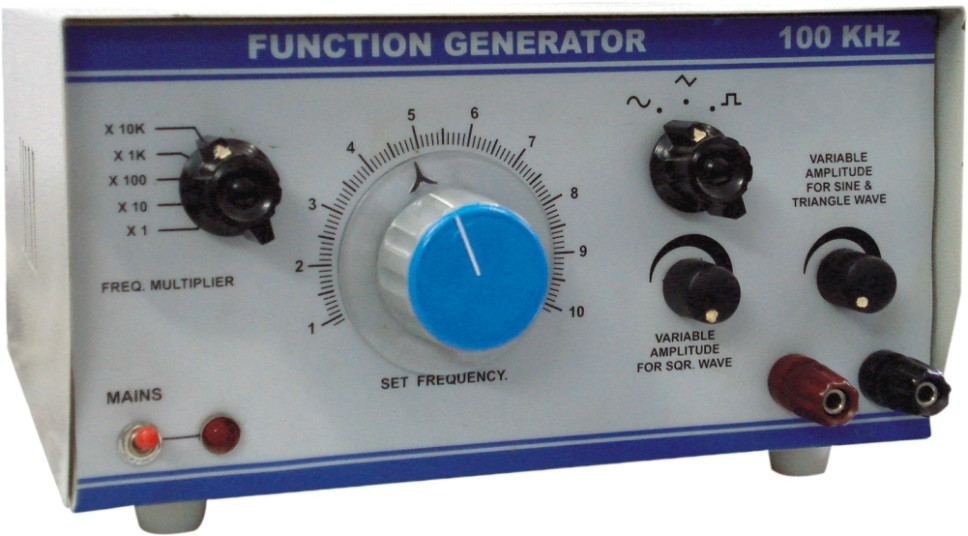
\includegraphics[width=.8\textwidth]{photos/function_generator.jpg}\\
\textsl{Photograph by Audin on Flickr.com}\\
\end{center}
\end{minipage}



\begin{minipage}{.5\textwidth}

\textbf{Oscilloscope} \\
The microphone can then pick up the sound and convert it to an electrical signal which can be displayed on the oscilloscope.\\
 
The most common oscilloscope controls are for amplitude, frequency, triggering, and channels. Once your teacher has helped you acquire a signal using the correct channel and triggering you will use the amplitude and frequency controls to display the characteristics of the sound being produced.\\
 
The amplitude adjustment of an oscilloscope controls how tall a given voltage will appear on the screen. The purpose of this adjustment is that you can see a very large or a very small signal on the same screen. \\

\end{minipage}
\begin{minipage}{.5\textwidth}
\begin{center}
\textbf{An oscilloscope}\\
\includegraphics[width=.8\textwidth]{photos/oscilloscope_Audin_Flickr.jpg}\\
\textsl{Photograph by Audin on Flickr.com}\\
\textbf{Two different oscilloscope traces}\\
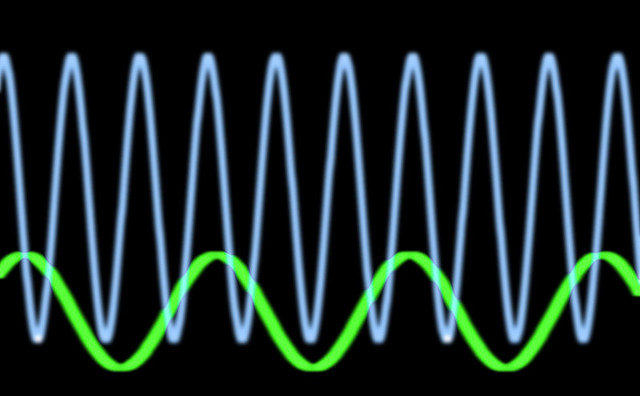
\includegraphics[width=.8\textwidth]{photos/oscilloscopetrace_Creativity103_Flickr.jpg}\\
\textsl{Photograph by Audin on Flickr.com}\\
\end{center}
\end{minipage}

\begin{minipage}{.5\textwidth}
 	
 	   The frequency (or time) adjustment of an oscilloscope is how much time will a certain distance across the screen represent. The purpose of this adjustment is to be able to see a very quickly changing or a slowly changing signal on the same screen. \\
\end{minipage}
\begin{minipage}{.5\textwidth}
\begin{center}
\begin{minipage}{.8\textwidth}
\vspace{.5cm}\textsl{\textbf{Note:} The display of the oscilloscope will show you a transverse wave pattern. This does not mean that sound waves are transverse waves but just shows that the pressure being measured is fluctuating because of a pressure wave.}
\end{minipage}
\end{center}
\end{minipage}
\vspace{1em}\\
You will be able to experiment with different amplitudes and frequencies using the function generator and see what impact the changes have on the waveform picked up by the microphone.\\
\end{activity}
\mindsetvid{Veritasium Ruben's tube}{VPebn}

            \section*{Intensity of sound [NOT IN CAPS]}
            \nopagebreak

	\par
      \label{m38800*id184075}Intensity is one indicator of amplitude. Intensity is the energy transmitted over a unit of area each second.\par 
\label{m38800*id184185}The unit of intensity is the \textbf{decibel} (symbol: dB).

\begin{table}[H]
\begin{center}
\begin{tabular}{|l|c|c|}\hline
\textbf{Source}&\textbf{Intensity} (dB) & \textbf{Times greater than hearing threshold}\\\hline
Rocket Launch &180 & $10^{18}$\\
Jet Plane & 140 & $10^{14}$ \\
Threshold of Pain & 120 & $10^{12}$\\
Rock Band & 110 & $10^{11}$\\
%Subway Train & 90 & $10^{9}$\\
Factory & 80 & $10^{8}$\\
City Traffic & 70 & $10^{7}$\\
Normal Conversation & 60 & $10^{6}$\\
Library & 40 & $10^{4}$\\
Whisper & 20 & $10^{2}$\\
Threshold of hearing & 0 & 0\\
\hline
\end{tabular}
\end{center}
\caption{Examples of sound intensities.}
\label{p:wsl:s11:intensity}
\end{table}

Vuvuzelas feature prominently at soccer events in South Africa. The intensity of the sound from a vuvuzela depends on how close you are. In Table~\ref{table:vuvuzelas} you can see how the intensity differs.

\begin{minipage}{.5\textwidth}
\begin{table}[H]
\begin{tabular}{ccccc}\hline
Frequency (Hz) & At ear & Bell opening & 1 m & 2 m \\ \hline
125&   36  	&62	 &38	& 35 \\ \hline
250&	92 &	106	& 82	&	 85 \\ \hline
500&	103 & 121&	 102&	 101 		\\ \hline
1 000&	106 & 122&	 108&	 100 	\\  \hline
2 000&	101 & 122&	 110&	 101 	\\ \hline
4 000&	97 & 109&	 110&	 102 	\\ \hline
5 000&	93 & 111&	 109&	 100 		\\ \hline
8 000&  87 & 110&	 107&		 98 	\\ \hline
\end{tabular}
\label{table:vuvuzelas}
\caption{Average vuvuzela intensity measurements across frequencies at 4 distinct distances from the bell end of the vuvuzela (dBA) taken from South African Medical Journal (Cape Town, South Africa) \textbf{100} (4): 192}
\end{table}
\end{minipage}
\begin{minipage}{.5\textwidth}
\begin{center}
\textbf{Vuvuzelas in action}\par
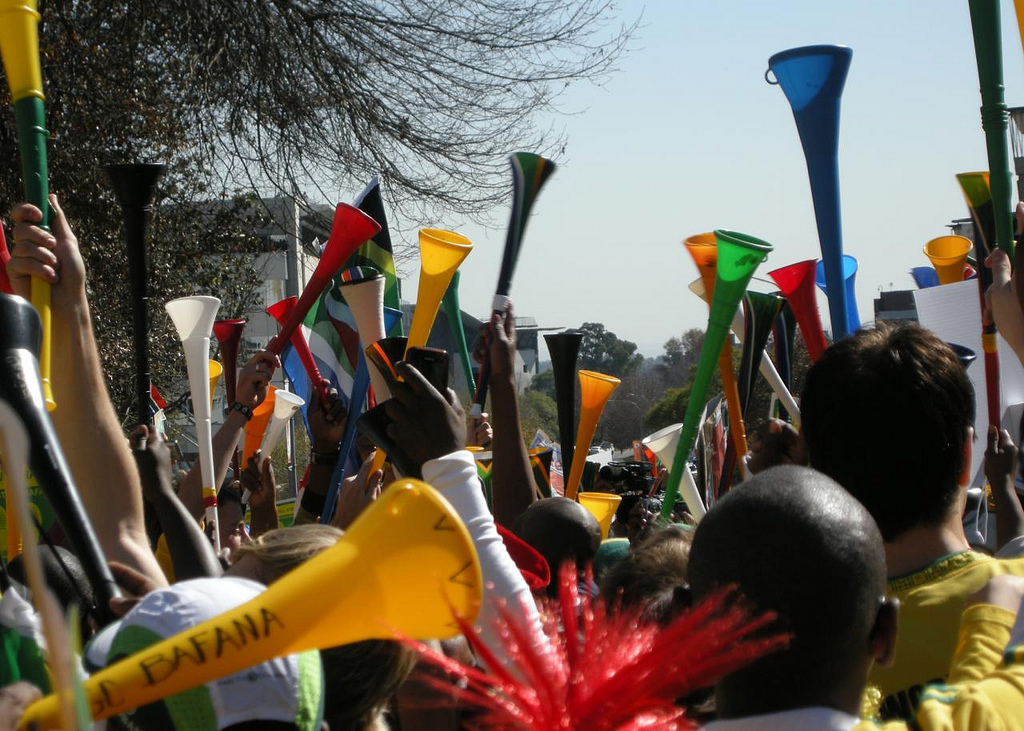
\includegraphics[width=.8\columnwidth]{photos/vuvuzelas_dundas_football_club.jpg}\par
Photo by Dundas Football Club on Flickr.com
\end{center}
\end{minipage}

    \label{m38800*cid6}
            \section{Ultrasound}
            \nopagebreak
      \label{m38800*id185135}Ultrasound is sound with a frequency that is higher than 20 kHz. Some animals, such as dogs, dolphins, and bats, have an upper limit that is greater than that of the human ear and can hear ultrasound.
    % \textbf{m38800*eip-558}\par
          \begin{table}[H]
    % \begin{table}[H]
    % \\ '' '0'
        \begin{center}
      \label{m38800*eip-558}
    \noindent
      \begin{tabular}{|l|c|c|}\hline
        Application &
        Lowest Frequency (kHz) &
        Highest Frequency (kHz) \\ \hline
        Cleaning (e.g. jewellery) &
        20 &
        40 \\ \hline
        Material testing for flaws &
        50 &
        500 \\ \hline
        Welding of plastics &
        15 &
        40 \\ \hline
        Tumour ablation &
        250 &
        2000 \\ \hline
    \end{tabular}
      \end{center}
    \caption{Different uses of ultrasound and the frequencies applicable.}
\end{table}
    \par
  \par 

\begin{minipage}{.5\textwidth}
\begin{center}
\textbf{Ultrasound image of a unborn baby}\par
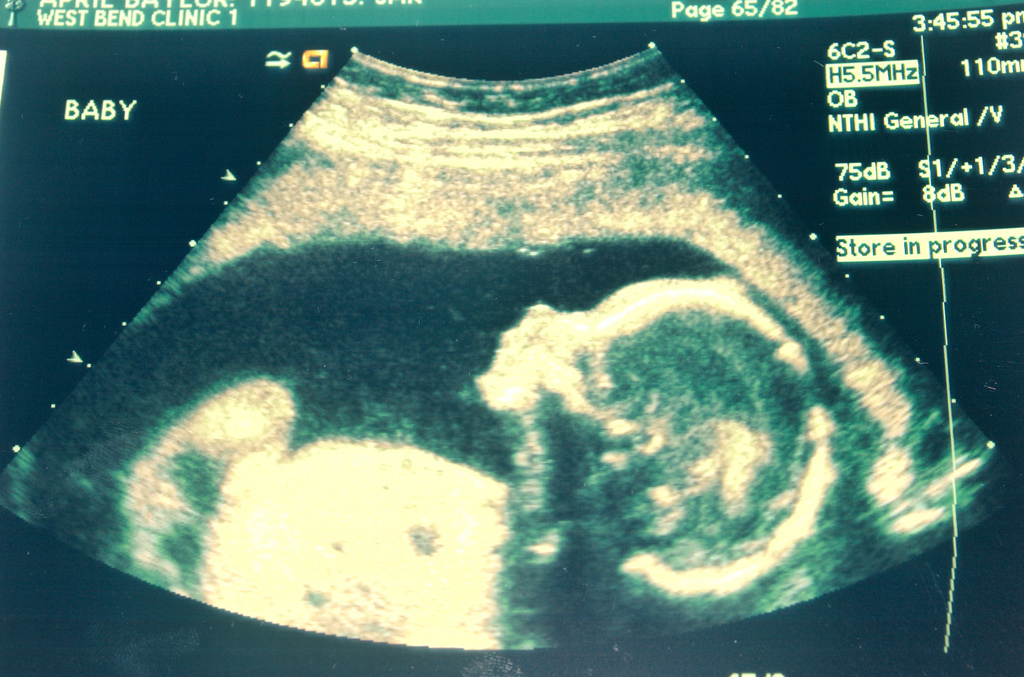
\includegraphics[width=.8\columnwidth]{photos/ultrasound_mbaylor_flickr.jpg}
\par\textit{Picture by mbaylor on Flickr.com}
\end{center}
\end{minipage}
\begin{minipage}{.5\textwidth}
      \label{m38800*id185140}The most common use of ultrasound is to create images, and has industrial and medical applications. The use of ultrasound to create images is based on the reflection and transmission of a wave at a boundary (when the wave goes from one substance to another). When an ultrasound wave travels inside an object that is made up of different materials such as the human body, each time it encounters a boundary, e.g. between bone and muscle, or muscle and fat, part of the wave is reflected and part of it is transmitted. The reflected rays are detected and used to construct an image of the object.\par 
      \label{m38800*id185148}Ultrasound in medicine can visualise muscle and soft tissue, making them useful for scanning the organs, and is commonly used during pregnancy. Ultrasound is a safe, non-invasive method of looking inside the human body.\par 
      
\end{minipage}
\IFact{Ultrasound generator\-/\-speaker systems are sold with claims that they frighten away rodents and insects, but there is no scientific evidence that the devices work; controlled tests have shown that rodents quickly learn that the speakers are harmless.}

\label{m38800*id185154}Ultrasound sources may be used to generate local heating in biological tissue, with applications in physical therapy and cancer treatment. Focused ultrasound sources may be used to break up kidney stones.\par 
      \label{m38800*id185159}Ultrasonic cleaners, sometimes called supersonic cleaners, are used at frequencies from 20-40 kHz for jewellery, lenses and other optical parts, watches, dental instruments, surgical instruments and industrial parts.
These cleaners consist of containers with a fluid in which the object to be cleaned is placed. Ultrasonic waves are then sent into the fluid. The main mechanism for cleaning action in an ultrasonic cleaner is actually the energy released from the collapse of millions of microscopic bubbles occurring in the liquid of the cleaner.\par 
\label{m38800*notfhsst!!!underscore!!!id482}


\section*{The physics of hearing [NOT IN CAPS]}
            \nopagebreak
\begin{figure}[H]
\begin{center}
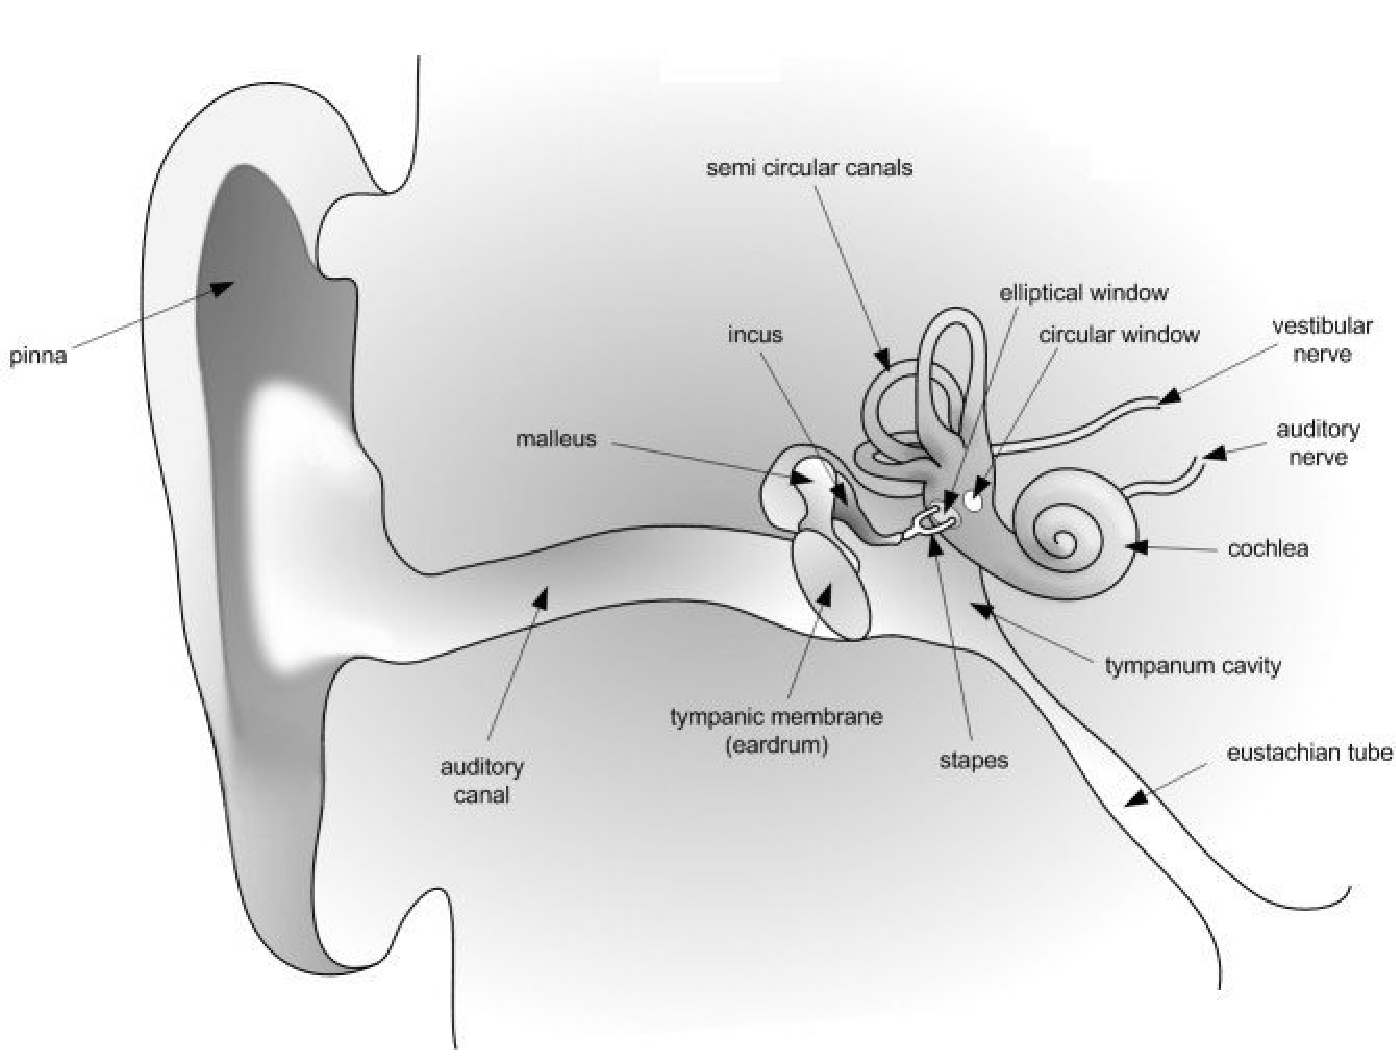
\includegraphics[width=0.65\textwidth]{HumanEar-GrayScale.pdf}
\end{center}
\caption{Diagram of the human ear. }
\label{Human Ear}
\end{figure}


      \label{m38800*id184052}The human ear is divided into three main sections: the outer, middle,
and inner ear. Let's follow the journey of a sound wave from the pinna (outermost part) to the auditory nerve (innermost part) which transmits a signal to the brain. The pinna is the part of the ear we typically think of when we refer to the ear. Its main
function is to collect and focus a sound wave. The wave
then travels through the ear canal until it meets the eardrum. The
pressure fluctuations of the sound wave make the eardrum vibrate.
The three very small bones of the middle ear, the malleus (hammer),
the incus (anvil), and the stapes (stirrup), transmit the signal through
to the elliptical window. The elliptical window is the beginning of the
inner ear. From the elliptical window the sound waves are transmitted through the liquid
in the inner ear and interpreted as sounds by the brain.
The inner ear, made of the semicircular canals, the cochlea,
and the auditory nerve, is filled with fluid. The fluid allows the body to
detect quick movements and maintain balance. 


%     \begin{equation}
%     \frac{\text{Joules}}{\text{s}\ensuremath{\cdot}{\text{m}}^{2}}=\frac{\text{Watts}}{{\text{m}}^{2}}
%       \end{equation}
%         \label{m38800*id184185}The unit of intensity is the \textbf{decibel} (symbol: dB). This reduces to an SI equivalent of $\text{W}\ensuremath{\cdot}{\text{m}}^{-2}$.\par 
%         \label{m38800*id184220}The average threshold of hearing is ${10}^{-12}\phantom{\rule{3.33333pt}{0ex}}\text{W}\ensuremath{\cdot}{\text{m}}^{-2}$. Below this intensity, the sound is too soft for the ear to hear. The threshold of pain is $1.0\phantom{\rule{3.33333pt}{0ex}}\text{W}\ensuremath{\cdot}{\text{m}}^{-2}$. Above this intensity a sound is so loud it becomes uncomfortable for
% the ear.\par 
%         \label{m38800*id184300}Notice that there is a factor of ${10}^{12}$ between the thresholds of
% hearing and pain. This is one reason we define the decibel (dB) scale.\par 
%         \label{m38800*id184613}In this way we can compress the whole hearing intensity scale into a
% range from 0 dB to 120 dB.\par 
%   \begin{table}[H]
% \begin{center}
% \begin{tabular}{|l|c|c|}\hline
% \textbf{Source}&\textbf{Intensity} (dB) & \textbf{Times greater than hearing threshold}\\\hline
% & & \\
% Rocket Launch &180 & $10^{18}$\\
% Jet Plane & 140 & $10^{14}$ \\
% Threshold of Pain & 120 & $10^{12}$\\
% Rock Band & 110 & $10^{11}$\\
% Subway Train & 90 & $10^{9}$\\
% Factory & 80 & $10^{8}$\\
% City Traffic & 70 & $10^{7}$\\
% Normal Conversation & 60 & $10^{6}$\\
% Library & 40 & $10^{4}$\\
% Whisper & 20 & $10^{2}$\\
% Threshold of hearing & 0 & 0\\
% \hline
% \end{tabular}
% \end{center}
% \caption{Examples of sound intensities.}
% \label{p:wsl:s11:intensity}
% \end{table}
    \par
        \label{m38800*id185097}There are sounds which exceed the threshold
of pain. Exposure to these sounds can cause immediate damage to hearing.
In fact, exposure to sounds from
80 dB and above can damage hearing over time. Measures
can be taken to avoid damage, such as wearing earplugs
or ear muffs. Limiting exposure time and
increasing distance between you and the source are also
important steps for protecting your hearing.\par 
\label{m38800*secfhsst!!!underscore!!!id469}

\begin{groupdiscussion}{Importance of Safety Equipment }
\label{m38800*id185111}Working in groups of 5, discuss the importance of safety equipment such as ear protectors for workers in loud environments, e.g. those who use jack hammers or direct aeroplanes to their parking bays. Write up your conclusions in a one page report. Some prior research into the importance of safety equipment might be necessary to complete this group discussion. 
\end{groupdiscussion} 
            \summary{VPecu}
            \nopagebreak
      \label{m38800*id185628}\begin{enumerate}[noitemsep, label=\textbf{\arabic*}. ] 
            \label{m38800*uid14}\item Sound waves are longitudinal waves
\label{m38800*uid15}\item The \textbf{frequency} of a sound is an indication of how high or low the \textsl{pitch} of the sound is.
\label{m38800*uid16}\item The human ear can hear frequencies from 20 to 20~000 Hz.
\textbf{Infrasound} waves have frequencies lower than 20 Hz.
\textbf{Ultrasound} waves have frequencies higher than 20~000 Hz.
\label{m38800*uid17}\item The \textbf{amplitude} of a sound determines its \textsl{loudness} or volume.
\label{m38800*uid18}\item The \textbf{tone} is a measure of the \textsl{quality} of a sound wave.
\label{m38800*uid19}\item The speed of sound in air is around $340\phantom{\rule{2pt}{0ex}}\text{m}\ensuremath{\cdot}\text{s}{}^{-1}$. It is dependent on the temperature, height above sea level and the phase of the medium through which it is travelling.
\label{m38800*uid20}\item Sound travels faster when the medium is hot.
\label{m38800*uid21}\item Sound travels faster in a solid than a liquid and faster in a liquid than in a gas.
\label{m38800*uid22}\item Sound travels faster at sea level where the air pressure is higher.
\label{m38800*uid23}\item The intensity of a sound is the energy transmitted over a certain area. Intensity is a measure of frequency.
\label{m38800*uid24}\item Ultrasound can be used to form pictures of things we cannot see, like unborn babies or tumours.
\label{m38800*uid25}\item Echolocation is used by animals such as dolphins and bats to ``see'' their surroundings by using ultrasound.
\label{m38800*uid26}\item Ships use sonar to determine how deep the ocean is or to locate shoals of fish.
\end{enumerate}

%\begin{table}[H]
%\begin{center}
%\begin{tabular}{|l|c|c|c|}\hline \hline 
%\multicolumn{4}{|c|}{\textbf{Units}}\\ \hline \hline
%\textbf{Quantity} & \textbf{Symbol} & \textbf{Unit} & \textbf{S.I. Units}\\ \hline
%Velocity & $v$ & \multicolumn{2}{|c|}{$\text{m}\cdot\text{s}^{-1}$} \\ \hline
%Wavelength & $\lambda$ & \multicolumn{2}{|c|}{m} \\ \hline
%Amplitude & $A$ & \multicolumn{2}{|c|}{m} \\ \hline
%Period & $T$ & \multicolumn{2}{|c|}{s} \\ \hline
%Frequency & $f$ & Hz & s$^{-1}$ \\ \hline
%\end{tabular}
%\end{center}
%\caption{Units used in \textbf{sound} }
%\label{table:sound::units}
%\end{table} 

\begin{table}[H]
\begin{center}
\begin{tabular}{|l|c|c|}\hline \hline 
\multicolumn{3}{|c|}{\textbf{Physical Quantities}}\\ \hline \hline
\multicolumn{1}{|c|}{\textbf{Quantity}} & \textbf{Unit name} & \textbf{Unit symbol}\\ \hline
Velocity ($v$) & metre per second & $\text{m} \cdot \text{s}^{-1}$ \\ \hline
Wavelength ($\lambda$) & metre & m \\ \hline
Amplitude ($A$) & metre & m \\ \hline
Period ($T$) & second & s \\ \hline
Frequency ($f$) & hertz & Hz \ \ ($s^{-1}$) \\ \hline
\end{tabular}
\end{center}
\caption{Units used in \textbf{sound} }
\label{table:sound::units}
\end{table}













\begin{eocexercises}{Sound}
            \nopagebreak
      \label{m38800*id185882}\begin{enumerate}[noitemsep, label=\textbf{\arabic*}. ] 
            \label{m38800*uid27}\item Choose a word from column B that best describes the concept in column A.
    % \textbf{m38800*id185898}\par
          \begin{center}
\begin{tabular}{ll}
\textbf{Column A} & \textbf{Column B} \\ \hline
1. pitch of sound \ \ \ & A. amplitude \\
2. loudness of sound \ \ \ \ \ \ \ \ \ & B. frequency \\
3. quality of sound \ \ \ & C. speed \\
& D. waveform \\
\end{tabular}
\end{center}
    \par
          \label{m38800*uid28}\item A tuning fork, a violin string and a loudspeaker are producing sounds. This is because they are all in a state of:
\label{m38800*id185988}\begin{enumerate}[noitemsep, label=\textbf{\alph*}. ] 
            \label{m38800*uid29}\item compression
\label{m38800*uid30}\item rarefaction
\label{m38800*uid31}\item rotation
\label{m38800*uid32}\item tension
\label{m38800*uid33}\item vibration
\end{enumerate}
                \label{m38800*uid34}\item What would a drummer do to make the sound of a drum give a note of lower pitch?
\label{m38800*id186066}\begin{enumerate}[noitemsep, label=\textbf{\alph*}. ] 
            \label{m38800*uid35}\item hit the drum harder
\label{m38800*uid36}\item hit the drum less hard
\label{m38800*uid37}\item hit the drum near the edge
\label{m38800*uid38}\item loosen the drum skin
\label{m38800*uid39}\item tighten the drum skin
\end{enumerate}
                \label{m38800*uid40}\item What is the approximate range of audible frequencies for a healthy human?
\label{m38800*id186144}\begin{enumerate}[noitemsep, label=\textbf{\alph*}. ] 
            \label{m38800*uid41}\item 0.2 Hz $\to $ 200 Hz
\label{m38800*uid42}\item 2 Hz $\to $ 2 000 Hz
\label{m38800*uid43}\item 20 Hz $\to $ 20 000 Hz
\label{m38800*uid44}\item 200 Hz $\to $ 200 000 Hz
\label{m38800*uid45}\item 2 000 Hz $\to $ 2 000 000 Hz
\end{enumerate}
                \label{m38800*uid46}\item X and Y are different wave motions. In air, X travels much faster than Y but has a much shorter wavelength. Which types of wave motion could X and Y be?
    % \textbf{m38800*id186268}\par
          \begin{table}[H]
    % \begin{table}[H]
    % \\ 'id2920184' '1'
        \begin{center}
      \label{m38800*id186268}
    \noindent
      \begin{tabular}{|l|l|l|}\hline
         &
        \uline{X} &
        \uline{Y} \\ \hline
        1. &
        microwaves &
        red light \\ \hline
        2. &
        radio &
        infra red \\ \hline
        3. &
        red light &
        sound \\ \hline
        4. &
        sound &
        ultraviolet \\ \hline
        5. &
        ultraviolet &
        radio \\ \hline
    \end{tabular}
      \end{center}
\end{table}
    \par
          \label{m38800*uid47}\item Astronauts are in a spaceship orbiting the moon. They see an explosion on the surface of the moon. Why can they not hear the explosion?
\label{m38800*id186399}\begin{enumerate}[noitemsep, label=\textbf{\alph*}. ] 
            \label{m38800*uid48}\item explosions do not occur in space
\label{m38800*uid49}\item sound cannot travel through a vacuum
\label{m38800*uid50}\item sound is reflected away from the spaceship
\label{m38800*uid51}\item sound travels too quickly in space to affect the ear drum
\label{m38800*uid52}\item the spaceship would be moving at a supersonic speed
\end{enumerate}
                \label{m38800*uid53}\item A man stands between two cliffs as shown in the diagram and claps his hands once.
    \setcounter{subfigure}{0}
	\begin{figure}[H] % horizontal\label{m38800*id186481}
   \begin{center}
{
\begin{pspicture}(0,-1.0985937)(7.6665626,1.1185937)
\psline[linewidth=0.04cm](1.260625,0.92140627)(1.260625,-1.0785937)
\psline[linewidth=0.04cm](6.260625,0.94140625)(6.260625,-1.0585938)
%\usefont{T1}{ptm}{m}{n}
\rput(0.4575,0.47140625){cliff 1}
%\usefont{T1}{ptm}{m}{n}
\rput(7.1339064,0.49140626){cliff 2}
\psline[linewidth=0.04cm](1.260625,-1.0785937)(6.240625,-1.0585938)
\psline[linewidth=0.04cm](4.260625,0.88140625)(4.240625,0.52140623)
\psline[linewidth=0.04cm,arrowsize=0.1029cm 2.04,arrowlength=1.44,arrowinset=0.4]{<->}(1.240625,0.70140624)(4.240625,0.70140624)
\psline[linewidth=0.04cm,arrowsize=0.0929cm 2.05,arrowlength=1.45,arrowinset=0.4]{<->}(4.300625,0.70140624)(6.260625,0.70140624)
\pscircle[linewidth=0.04,dimen=outer](4.250625,0.21140625){0.25}
\psline[linewidth=0.04cm](4.240625,-0.05859375)(4.240625,-0.6585938)
\psline[linewidth=0.04cm](4.240625,-0.6585938)(3.940625,-1.0585938)
\psline[linewidth=0.04cm](4.240625,-0.6585938)(4.540625,-1.0585938)
\psline[linewidth=0.04cm](4.040625,-0.25859374)(4.440625,-0.25859374)
%\usefont{T1}{ptm}{m}{n}
\rput(2.6015625,0.94140625){\footnotesize 165 m}
%\usefont{T1}{ptm}{m}{n}
\rput(5.2015624,0.94140625){\footnotesize 110 m}
\end{pspicture}
}
\end{center}
 \end{figure}       
Assuming that the velocity of sound is $330\phantom{\rule{2pt}{0ex}}\text{m}\ensuremath{\cdot}\text{s}{}^{-1}$, what will be the time interval between the two loudest echoes?
\label{m38800*id186509}\begin{enumerate}[noitemsep, label=\textbf{\alph*}. ] 
            \label{m38800*uid54}\item $\frac{2}{3}\phantom{\rule{2pt}{0ex}}\text{s}$
\label{m38800*uid55}\item $\frac{1}{6}\phantom{\rule{2pt}{0ex}}\text{s}$
\label{m38800*uid56}\item $\frac{5}{6}\phantom{\rule{2pt}{0ex}}\text{s}$
\label{m38800*uid57}\item 1 s
\label{m38800*uid58}\item $\frac{1}{3}\phantom{\rule{2pt}{0ex}}\text{s}$
\end{enumerate}
                \label{m38800*uid59}\item A dolphin emits an ultrasonic wave with frequency of 0,15 MHz. The speed of the ultrasonic wave in water is $1 500\phantom{\rule{2pt}{0ex}}\text{m}\ensuremath{\cdot}\text{s}{}^{-1}$. What is the wavelength of this wave in water?
\label{m38800*id186650}\begin{enumerate}[noitemsep, label=\textbf{\alph*}. ] 
            \label{m38800*uid60}\item 0,1 mm
\label{m38800*uid61}\item 1 cm
\label{m38800*uid62}\item 10 cm
\label{m38800*uid63}\item 10 m
\label{m38800*uid64}\item 100 m
\end{enumerate}
                \label{m38800*uid65}\item The amplitude and frequency of a sound wave are both increased. How are the loudness and pitch of the sound affected?
    % \textbf{m38800*id186726}\par
          \begin{table}[H]
    % \begin{table}[H]
    % \\ 'id2920575' '1'
        \begin{center}
      \label{m38800*id186726}
    \noindent
      \begin{tabular}{|l|l|l|}\hline
         &
        \uline{loudness} &
        \uline{pitch} \\ \hline
        A &
        increased &
        raised \\ \hline
        B &
        increased &
        unchanged \\ \hline
        C &
        increased &
        lowered \\ \hline
        D &
        decreased &
        raised \\ \hline
        E &
        decreased &
        lowered \\ \hline
    \end{tabular}
      \end{center}
\end{table}
    \par
          \label{m38800*uid66}\item A jet fighter travels slower than the speed of sound. Its speed is said to be:
\label{m38800*id186857}\begin{enumerate}[noitemsep, label=\textbf{\alph*}. ] 
            \label{m38800*uid67}\item Mach 1
\label{m38800*uid68}\item supersonic
\label{m38800*uid69}\item subsonic
\label{m38800*uid70}\item hypersonic
\label{m38800*uid71}\item infrasonic
\end{enumerate}
                \label{m38800*uid72}\item A sound wave is different from a light wave in that a sound wave is:
\label{m38800*id186936}\begin{enumerate}[noitemsep, label=\textbf{\alph*}. ] 
            \label{m38800*uid73}\item produced by a vibrating object and a light wave is not.
\label{m38800*uid74}\item not capable of travelling through a vacuum.
\label{m38800*uid75}\item not capable of diffracting and a light wave is.
\label{m38800*uid76}\item capable of existing with a variety of frequencies and a light wave has a single frequency.
\end{enumerate}
                \label{m38800*uid77}\item At the same temperature, sound waves have the fastest speed in:
\label{m38800*id187004}\begin{enumerate}[noitemsep, label=\textbf{\alph*}. ] 
            \label{m38800*uid78}\item rock
\label{m38800*uid79}\item milk
\label{m38800*uid80}\item oxygen
\label{m38800*uid81}\item sand
\end{enumerate}
                \label{m38800*uid82}\item Two sound waves are travelling through a container of nitrogen gas. The first wave has a wavelength of 1,5~m, while the second wave has a wavelength of 4,5~m. The velocity of the second wave must be:
\label{m38800*id187073}\begin{enumerate}[noitemsep, label=\textbf{\alph*}. ] 
            \label{m38800*uid83}\item $\frac{1}{9}$ the velocity of the first wave.
\label{m38800*uid84}\item $\frac{1}{3}$ the velocity of the first wave.
\label{m38800*uid85}\item the same as the velocity of the first wave.
\label{m38800*uid86}\item three times larger than the velocity of the first wave.
\label{m38800*uid87}\item nine times larger than the velocity of the first wave.
\end{enumerate}
%                 \label{m38800*uid88}\item Sound travels at a speed of 340~m$\ensuremath{\cdot}$s${}^{-1}$. A straw is 0,25 m long. The standing wave set up in such a straw with one end closed has a wavelength of 1,0~m. The standing wave set up in such a straw with both ends open has a wavelength of 0,50 m.
% \label{m38800*id187205}\begin{enumerate}[noitemsep, label=\textbf{\alph*}. ] 
%             \label{m38800*uid89}\item calculate the frequency of the sound created when you blow across the straw with the bottom end closed.
% \label{m38800*uid90}\item calculate the frequency of the sound created when you blow across the straw with the bottom end open.
% \end{enumerate}
                \label{m38800*uid91}\item A lightning storm creates both lightning and thunder. You see the lightning almost immediately since light travels at $3\ensuremath{\times}{10}^{8}\phantom{\rule{0.166667em}{0ex}}\text{m}\ensuremath{\cdot}{\text{s}}^{-1}$. After seeing the lightning, you count 5~s and then you hear the thunder. Calculate the distance to the location of the storm.\newline
\label{m38800*uid92}\item A person is yelling from a second story window to another person standing at the garden gate, 50~m away. If the speed of sound is 344~m$\ensuremath{\cdot}$s${}^{-1}$, how long does it take the sound to reach the person standing at the gate?\newline
% \label{m38800*uid93}\item A piece of equipment has a warning label on it that says, "Caution! This instrument produces 140 decibels." What safety precaution should you take before you turn on the instrument?\newline
% \label{m38800*uid94}\item What property of sound is a measure of the amount of energy carried by a sound wave?\newline
\label{m38800*uid96}\item Person 1 speaks to person 2. Explain how the sound is created by person 1 and how it is possible for person 2 to hear the conversation.\newline
\label{m38800*uid97}\item Sound cannot travel in space. Discuss what other modes of communication astronauts can use when they are outside the space shuttle?\newline
\label{m38800*uid98}\item An automatic focus camera uses an ultrasonic sound wave to focus on objects. The camera sends out sound waves which are reflected off distant objects and return to the camera. A sensor detects the time it takes for the waves to return and then determines the distance an object is from the camera. If a sound wave (speed = 344~m$\ensuremath{\cdot}$s${}^{-1}$) returns to the camera 0,150~s after leaving the camera, how far away is the object?\newline
\label{m38800*uid99}\item Calculate the frequency (in Hz) and wavelength of the annoying sound made by a mosquito when it beats its wings at the average rate of 600 wing beats per second. Assume the speed of the sound waves is 344~m$\ensuremath{\cdot}$s${}^{-1}$.        
\label{m38800*uid100}\item How does halving the frequency of a wave source affect the speed of the waves?\newline
\label{m38800*uid101}\item Humans can detect frequencies as high as 20~000 Hz. Assuming the speed of sound in air is 344~m$\ensuremath{\cdot}$s${}^{-1}$, calculate the wavelength of the sound corresponding to the upper range of audible hearing.\newline
\label{m38800*uid102}\item An elephant trumpets at 10~Hz. Assuming the speed of sound in air is 344~m$\ensuremath{\cdot}$s${}^{-1}$, calculate the wavelength of this infrasonic sound wave made by the elephant.\newline
\label{m38800*uid103}\item A ship sends a signal out to determine the depth of the ocean. The signal returns 2,5 seconds later. If sound travels at
1450 m.s${}^{-1}$ in sea water, how deep is the ocean at that point?\newline
\label{m38783*uid44}\item A person shouts at a cliff and hears an echo from the cliff 1~s later. If the speed of sound is $344\phantom{\rule{2pt}{0ex}}\text{m}\ensuremath{\cdot}\text{s}{}^{-1}$, how far away is the cliff?\newline
\label{m38783*uid37}\item Select a word from Column B that best fits the description in Column A:
    % \textbf{m38783*id293899}\par
          \begin{center}
\begin{tabular}{ll}
\textbf{Column A} & \textbf{Column B} \\ \hline
1. waves in the air caused by vibrations & A. longitudinal waves \\
2. waves that move in one direction, but medium moves in another & B. frequency \\
3. waves and medium that move in the same direction & C. period \\
4. the distance between consecutive points of a wave which are in phase & D. amplitude \\
5. how often a single wavelength goes by & E. sound waves \\
6. half the difference between high points and low points of waves & F. standing waves \\
7. the distance a wave covers per time interval & G. transverse waves \\
8. the time taken for one wavelength to pass a point & H. wavelength \\
& I. music \\
& J. sounds \\
& K. wave speed \\
\end{tabular}
\end{center}
\end{enumerate}
  \label{m38800**end}
  \label{9b5d72dd5f0585e544578ab90a9956a8**end}
\par \practiceinfo
 \par \begin{tabular}[h]{cccccc}
 (1.) 003u  &  (2.) 003v  &  (3.) 003w  &  (4.) 003x  &  (5.) 003y  &  (6.) 003z  &  (7.) 0040  &  (8.) 0041  &  (9.) 0042  &  (10.) 0043  &  (11.) 0044  &  (12.) 0045  &  (13.) 0046  &  %(14.) 0047  Was removed!
  (14.) 0048  &  (15.) 0049  &  
%(16.) 004a  &  (17.) 004b  &  Original 17 and 18 removed
(16.) 004c  &  
(17.) 004d  &  (18.) 004e  &  (19.) 004f  &  (20.) 004g  &  (21.) 004h  &  (22.) 004i  &  (23.) 004j  & (24.) 004k & (25.) 004m  \end{tabular}

\end{eocexercises}
